\chapter{Manufacturing Systems}
	
	To give a shape shape to a block of raw material, namely \textit{\textbf{workpiece}}, various methods can be used involving a different required number of \de{motion axis}:
	\begin{itemize}
		\item the \textbf{forming} processes that are based on the plastic deformation of the workpiece requires at least 1 motion axis. In this course such manufacturing process is skipped because the motion planning and control is (usually) trivial;
		\item \textbf{subtractive} processes are based on the removal of material from the workpiece and usually requires 2.5 motion axis or more;
		\item we can add more material to the existing block using \textbf{additive manufacturing} techniques that, as for subtractive processes, requires at least 2.5 motion axis.
	\end{itemize}
	In subtractive/additive manufacturing there is a \de{tool} performing the process (such mills, polarized wires, extruding nozzles...) whose motion is performed by a synchronized action of two or more axes (typically in cartesian arrangement); the union of \textbf{trajectory} and \textbf{speed} of the tool represent it's \de{motion} that must be planned according to \textbf{geometry} and \textbf{process specifics}.
	
	
\section{Machining}
	
	The majority of products involves the \de{machining} process either directly or indirectly; machining involves a combination of linear and rotary motion and can be split in 3 main operational categories:
	\begin{itemize}
		\item \textbf{turning} where the workpiece is rotating and the tool is displacing; a good example of turning machining is the lathe (\textit{tornio});
		\item in \textbf{drilling} and \textbf{milling} the tool is rotating and there is a combined relative displacement between tool and workpiece.
	\end{itemize}
	The mechanism of \textbf{chip formation} (\textit{formazione di trucioli}) generated by this processes depends on multiple \textbf{tool parameters} such:
	\begin{itemize}
		\item the relative speed of the tool and the workpiece, namely the \textbf{cutting speed};
		\item the cross section of the removed material
	\end{itemize}
	This tool parameters strictly depends on the \textbf{machining parameters} as trajectory, rotation and translation speeds.
	
	\subsection*{Turning}
		
		While dealing with \textbf{turning}, considering the scheme in figure \ref{fig:man:turning}, the main machining parameters are the spindle speed, the feed rate and the spindle power.
		
		\begin{SCfigure}[2][bht]
			\centering 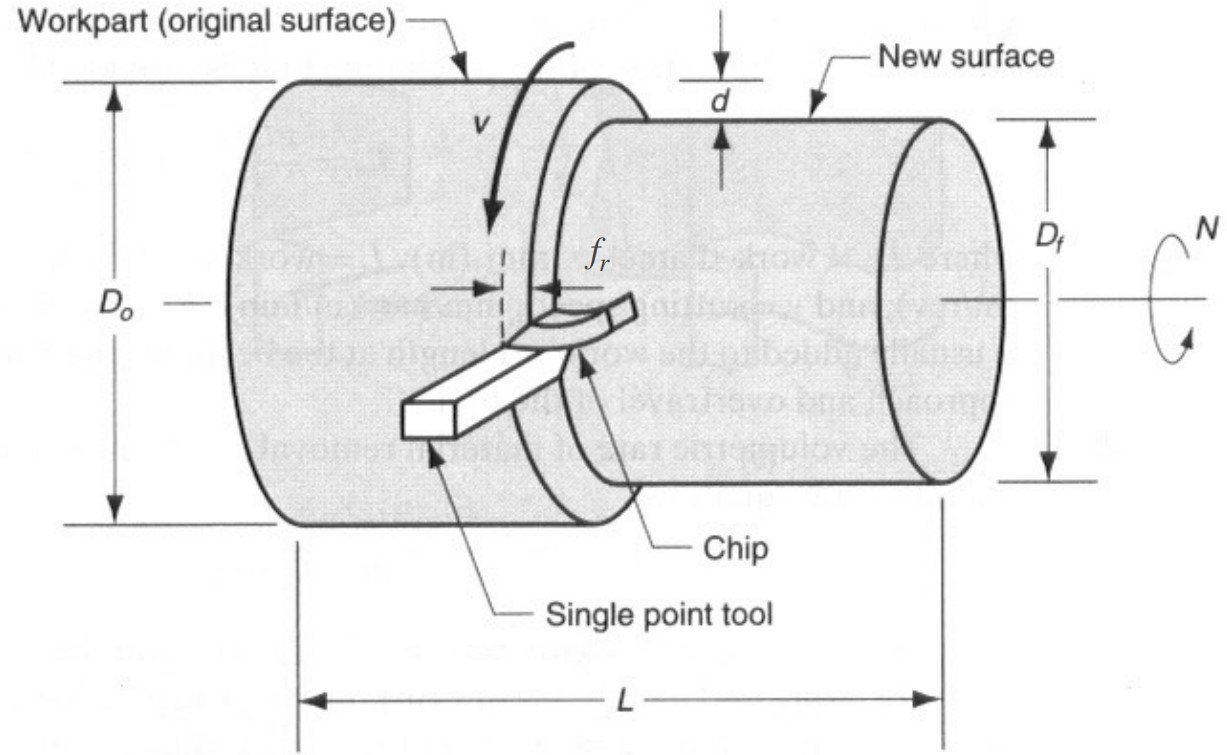
\includegraphics[width=7cm]{turning}
			\caption{main dimensions and parameters used for the calculation on turning's machining parameters.} \label{fig:man:turning}
		\end{SCfigure}
	
		
		
		\begin{table}[bht]
			\centering
			\tabrule
			\caption{formulas for machining systems} \vspace{2mm}
			\begin{tabular} {M{3cm} M{3cm} M{3cm} M{3cm}}
				Parameter  & Turning & Milling & Drilling \\ \hline
				$v(m/min)$ & $\pi D_0 N$ & $\pi D N$ & $\pi D N$ \\
				$N(1/min)$ & $\frac{v}{\pi D_0}$ & $\pi D N$ & $\pi D N$ \\
				
			\end{tabular}	
				
			\vspace{2mm}
			\tabrule
		\end{table}
	
	
	
	
	
	
	
	
	
	